\chapter{Referencial Teórico}

\section{Princípios e Padrões de Projetos}

Desenvolver software orientado a objetos é um desafio. Criar uma representação
computacional de uma faceta da realidade em que seus constituintes trabalhem de
forma horminiosa para atingir as necessidades que o software se propõe a
atender requer experiência, conhecimento do domínio do problema e um processo de
análise e projeto. Apesear de existir várias abordagens para se conceber um
sistema orientado a objetos\cite{evans2004ddd},\cite{gomma11} um sistema bem
contruído apresetam características fundamentais. Coesão, acoplamento etc

Um padrão dentro do contexto de estudo deste presente trablho pode ser definido
como uma técnica efetiva cuja a sua aplicabilidade é aceita e difundiida dentro
de uma área de conhecimento com a intenção de atingir um
objetivo\cite{MetskerWake06}.

Em densenvolvimento de software o catálogo mais difundido de padrões de projetos
orientado a objetos é elaborado por \citeonline{gof} contendo um total de 23
padrões formalmente documentados que acumulam experiências bem sucedidas em
diversos sistemas. Esses padrões tem a seguinte classificação:

\begin{description}
\item[Criacionais] Padrões que definem como criar novas instâncias de classes.
\item[Estruturais] Foca na estruturação das classes e objetos.
\item[Comportamentais] Definem como as classes e objetos interagem entre si e
suas responsabilidades.
\end{description}



%argumentação
Analisando a forma como um padrão de projeto é concebido definindo papéis de
cada elemento participante e como eles interagem entre se podemos concluir que
o uso dos padrões de projeto promove maior coesão, melhor separação de
interesses e baixo acoplamento no sistema. Todas essas características são muito
importantes contribuem para um software de melhor qualidade

%Melhorar isso

%Linkar com as metricas, mostrar relação metricas e padroes


\section{Métricas de qualidade OO}

Com o advento de novas técnicas de desenvolvimento de software é necessário
obter informações do impacto dessas inovações nos resultados de um projeto. Com
esse objetivo \citeonline{cksuite} elaborou um conjunto de métricas para mensurar a
qualidade de sistemas desenvolvido usando o paradigma orientado a objetos que
não se limitasse a uma linguagem de programação, fácil de coletar e com forte
embasamento teórico na ontologia de bunge. This model is used to analyze
some static and dynamic properties of an information system and to examine the
question of what constitutes a good decomposition of an information
system\cite{WandWeber}As métricas são:

%Bunge’s ontology has
%considerable appeal for 00 researchers since it deals with the
%meaning and definition of representations of the world, which
%are precisely the goals of the object oriented approach [32]



\begin{description}
\item[Acoplamento entre objetos (CBO)] Número de classes que ela depende por
meio da relação de composição. Uma classe está acoplada a outra quando o método
de um classe invoca o método de uma variável de instância de outra classe que
gera uma dependência entre essas classes, quanto maior essa dependência mais
difícil é reutilizar esses componetes em outras partes do sistema além do
aumento do risco de efeitos colaterais ocorrerem ao modificar uma classe
altamente acoplada.
\item[Ausência de coesão dos métodos(LCOM)] Usado para avaliar a coesão de uma
classe através da similaridade entre seus métodos. Um método tem similaridade
com outro quando a intercessão entre os conjuntos de atributos usados por ambos
os métodos tem cardinalidade maior que zero. LCOM mostra esses conjuntos nulos
indicando os métodos que usam esses atributos deveriam ser implementados em
outra classe. Essa similaridade expressa a coesão da classe.
\item[Profundidade na árvore de herança (DIT)] Nível de uma classe na
hierárquia de herança. Reflete o número máximo de elementos pai dentro da aŕvove
de classes até a raiz o que aumenta a complexidade conforme a quantidade de
elementos envolvidos se eleva, diminuindo a previsibilidade do comportamento da
classe com vários métodos e atributos sendo herdados, principalmente com o uso
de sobrecarga de métodos.
\item[Métodos por Classe (WMC)] Serve para expressar o nível de complexidade de
uma classe basseado no número de métodos que ela possui. Isso afeta o esforço de
manutenção da classe, além de impactar nas classe filhas que herdarão esses
métodos e também é um indicativo de a classe tem métodos espefíficos
dificultando o seu reuso.
\item[Número de classes filhas (NOC)] Número de subclasses imediatas de uma
classe. Essa medida é um indicativo de mau uso de herança conforme seu valor
aumenta e mostra o impacto que uma classe pode ter no sistema requerendo maior
atenção e testes.
\item[Response sets for Class (RFC)] Quantidade de métodos que são executados
quando um objeto recebe uma mensagem, incluindo os métodos de outras classes. 
\end{description}

Todas essas métricas tem uma relação inerentes com a coesão e acoplamento dos
objetos sendo uma forma ``confiável'' para a análise da qualidade em sistemas
orientados a objetos. Os aplicativos desenvolvidos para a plataforma android são
escritos usando a linguagem de programação java que emprega esse paradigma de
desenvolvimento, o que justifica o uso das métricas de \citeonline{cksuite} para
validação dos projetos orientados a objetos.



\section{Model View Controller}

O padrão Model View Controller surgiu como uma solução genérica para usuários
de uma sistema de planejamento manipulem dados complexos\citeonline{Reenskaug:1979}.
Posteriormente \citeonline{krasnerPope1988} implementam um framework MVC para o
ambiente gráfico da linguagem de programação Smalltalk-80 como uma forma de
promover a reusabilidade e plugabilidade.

Segundo \citeonline{Reenskaug:1979} o principal objetivo do MVC ``\ldots was to
support the user's mental model of the relevant information space and to enable
the user to inspect and edit this information.''. Esse modelo mental é como o
usuário percebe o dominio do problema que está inserido no qual executará suas
atividades sobre dados de seu interesse. Para que o usuário de um sistema de
informação possa interagir com a represetação computacional  de seu modelo
mental três componetes são definidos:

Models - É o compoente constituído de uma composição de classes que implementam
as regras de negócio referentes as funcionalidades que o programa provê,
representa o  conhecimento que o usuário tem e como manipula-lo. Atende
mensagens da view requisitando seu estado e mensagens do controller para mudar
seu estado,

Views - Representação específica de um model na interface com o usuário, é 
responsável por todo a manipulação visual, recuperando um estado do model e
exibindo os dados, podendo ser composta por sub-views e ser parte de views mais
complexas.

Controllers - Interpreta a as ações do usuário provenientes de um dispositivo de
entrada(Teclado, Mouse) alterando estado da view ou do model.




\citeonline{krasnerPope1988} descreve a estrutura do MVC onde a view tem seu
controller exclusivo mantendo uma dependência cíclica entre ambos e tanto a view
quanto o controller tem referências diretas para o model por meio de atributos
de classe porém o model não deve conhecer seus respectivos pares de
View-Controller para promover mais reuso de código e encapsulamento do model. As
alterações do estado do model são feitas na maioria das vezes pelo controller, e
o model é responsável por notificar todas as views que o representa para que
se atualizem refletindo o novo estado. No caso de um model ser usado por vários
pares de View-Controller as mensagens de notificação de um novo estado do model
podem ser parametrizadas assim cada view pode verificar se a alteração é de seu
interesse. Segundo \citeonline{Fowler:2002:PEA} ``Of these the separation of presentation
from model is one of the most fundamental heuristics of good software design''.

O controller poderia ser o responsável por publicar as alterações no estado do
model devido sua relação direta com o mesmo, mas em casos onde o model é
alterado por outro componente que não é um dos controladores que os utilizam, é
necessário que o model conheça as views que devem ser notificados do novo
estado. Para que essas alterações de estado sejam propagadas a view e o
controller são registrados como dependentes de seu model. O padrão é descrito
dentro do contexto no qual o surgiu levando em consideração caracteristicas
espefíficas da  linguagem de programação que dão suporte à implementação dos
três componentes como por exemplo o gerenciamento dos objetos que são
dependentes do model definido na classe Objet que o model deve extender. A
Figura \ref{mvc_seq} esclarece a interação entre os componetes.

\begin{figure}[h]
	\centering
	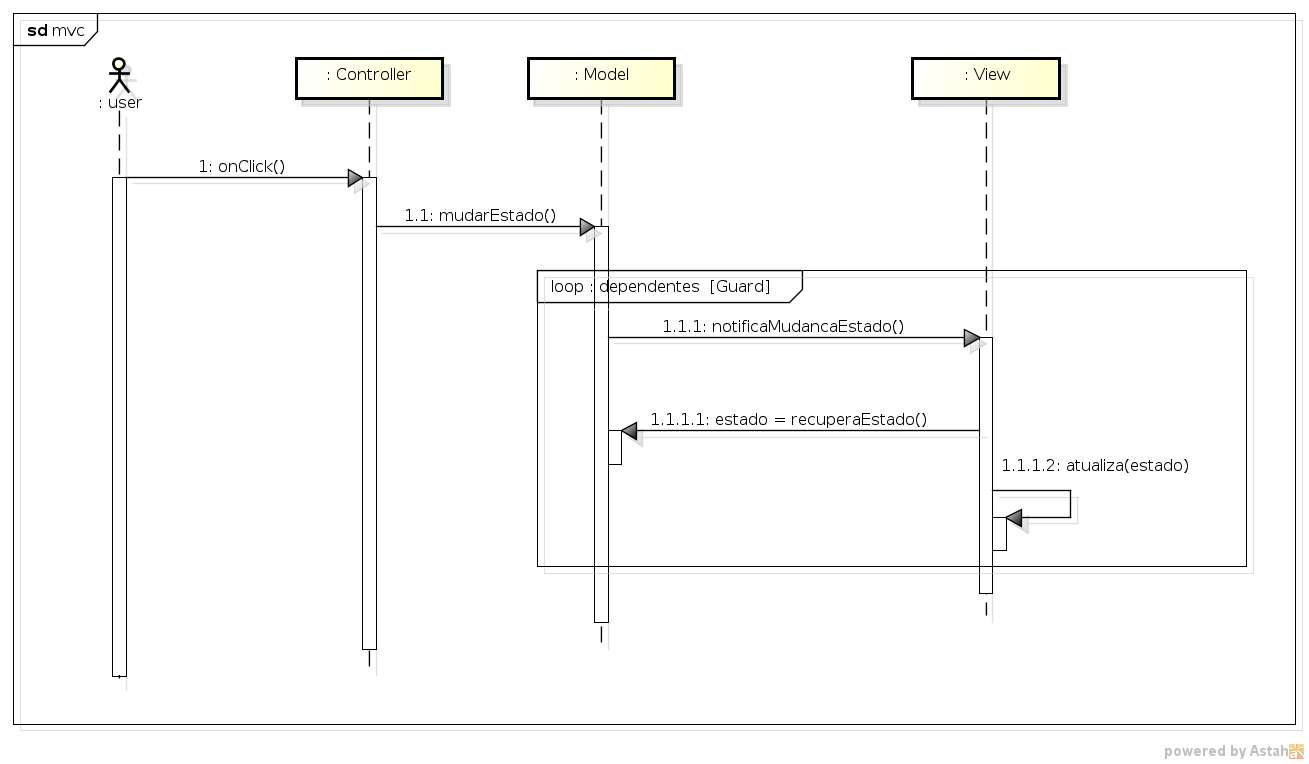
\includegraphics[scale=0.5]{img/mvc_seq.png}
	\caption{Diagrama de Sequência do MVC/Fonte: Próprio Autor}
	\label{mvc_seq}
\end{figure}

\citeonline{gof} cita \citeonline{krasnerPope1988} fazendo uma análise dos
objetos que compõem o MVC relacionando-os com outros padrões de proejtos
descritos em seu catálogo.
O desacoplamento entre a view e o model e a propagação das mudanças de estado no
model para os objetos regitrados como dependentes do model pode ser descrico
como uma implementação do padrão Observer. A hierarquia de views é um exemplos
de Composite pois uma view pode ser constituída por sub-views para compor views
complexas. O Strategy é aplicando ao controller que encapsula o algoritmo que
vai alterar a view e o model podendo ser substituído por uma outra
implementação que deixa de responder às interações com o usuário.

Segundo \citeonline{krasnerPope1988} o Model ``\ldots can be as simple as an integer
(as the model of a counter) or string (as the model of a text editor), or it can
be a complex object''. O model pode ser implementado usando o pardrão Facade
para simplificar as interações com o model dependendo da complexidade do
domínio que ele representa.
%citar facade aqui



\section{Model View Presenter}

O MVP é um modelo de programação para implementação de interfaces com o usuário
desevolvido como um framework para C++ e Java, criado por uma subsidiária da IBM
chamda Taligent,Inc. Este padrão é baseado no MVC e descreve vários componentes que tem as
responsabilidades de como gerenciar os dados da aplicação e como o usuário
interage com esses dados tendo como objetivo promover o encapsulamento do Model
, reuso de lógica de negócio e o polimorfismo da View.

\begin{description}
  \item[Model] Tem as mesmas responsabilidades que o Model definido pelo MVC.
  \item[Selections] - Abstração para selecionar um subconjunto dos dados
  existentes no model.
  \item [Commands] Representa as operações a serem executadas sobre uma
  Selection do Model.
  \item [View] Responsável por exibir o model assim como no MVC.
  \item [Interactor] Mapeia os interações do usuário na view como eventos do
  mouse.
  \item [Presenter] O papel do presenter é interpretar o eventos iniciados pelo
  usuário executando a lógica de negócio correspondente implementada em um
  command para manipular o model \cite{Potel96mvp}.
\end{description}


%interpretações do mvp
%Objectarts
Os conceitos do MVP são descritos em \citeonline{Potel96mvp} de forma genérica
permintindo interpretações para uma implementação efetiva.
\citeonline{twisttriad:2000} descreve a implementação de um framework para
Dolphin Smalltalk\footnote{Implementação da Linguagem de programação Smalltalk,
http://www.object-arts.com} adotando os conceitos do MVP onde salienta que a
maioria dos sistemas operacionais com ambiente gráfico fornece um conjunto de
componetes (Widgets) no qual está contido a responsbilidade do controller.A
maior parte do comportamento do caso com o usuário é implementada no
presenter que está diretamente associado a View

Ainda acerca das responsabilidades do presenter \citeonline{fowler:ui} descreve
o que é chamado de Passive View onde toda a lógica do comportamento da view é
implementado no presenter deixando a view enxuta com o intuito de isolar ao
máximo a api gráfica do resto da aplicação, permitindo uma maior cobertura de
testes aplicados ao presenter. Dessa forma o model não se comunica com a view
por meio do observer pattern, sendo que a view séra atualizada pelo presenter.


MVP se adequa melhor as apis gráficas existentes e define de forma mais clara os
componetes necessários para desenvolver uma aplicação, sendo o ponto de maior
discussão reside em quais os limites das responsabilidades no que tange a
mediação do Model e a View por parte do Presenter.


\section{Framework Android}
 

O android é um sistema operacional baseado no linux mantido pela Google para
ser embarcado em dispositivos podendo ser aplicado em carros, televisão, placas
controladoras mas seu destaque é a utilização em dispositivos smartphones e
tablet que é o foco deste trabalho.
A plataforma é contituída por uma pilha softwares e frameworks tendo em sua base
o sistema operacional e seu drivers seguido da máquina virtual que executa os
aplicativos android e bibliotecas auxiliares, SDK e ferramentas de
desenvolvimento e aplicativos básicos.

\begin{figure}[h]
	\centering
	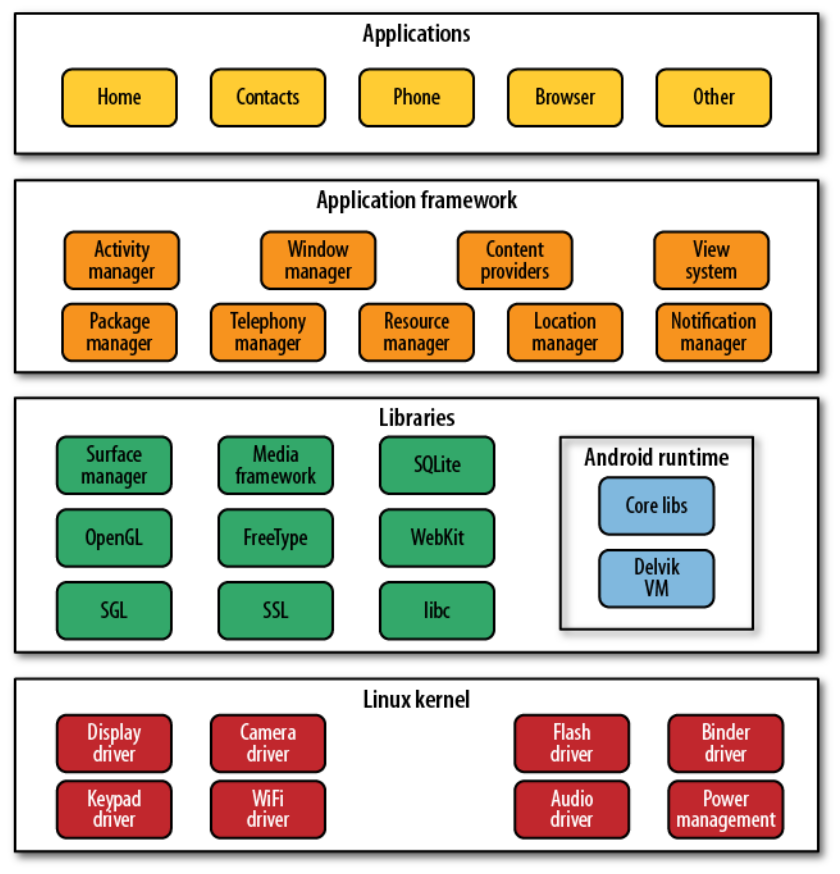
\includegraphics[scale=0.5]{img/android_stack.png}
	\caption{Android Stack/Fonte: Learning Android}
	\label{android_stack}
\end{figure}

Para desenvolvimento é usado a api disponível no sdk que define
os blocos de construção de um aplicativo:

\begin{description}
  \item[Activity] Representa uma atividade que o usuário executa no aplicativo
  em um determinado momento. Usado para criar a interface contém todos os
  componetes visuais e responde à interações do usuário.
  \item[Service] Responsável por executar uma operação sem interface gráfica
  indicado para processamentos longos como por exemplo a execução de uma música
  ou download de de arquivos.
  \item[Broadcast Receiver] Implementação do padrão publish/subscribe 
  \item[Content Provider] Usado para expor dados de uma aplicativo para outros
  aplicativos. Os dados podem ser provenientes de qualquer forma de
  armazenamento como um arquivo ou banco de dados.
  \item[ApplicationContext] Representa a aplicação em execução provendo acesso
  a recursos.
  \item[AsyncTask] Usado para implementar computação paralela evitando o uso da
  linha de execução principal do aplicativo que é respoonsável por tratar a
  interações com o usuário.
\end{description}


Com base nos componentes de framework e literatura revisada é possível fazer
uma análise dos mesmos e projetar uma camada de apresentação utilizando o padrão
MVP para ser usada como referência de implemntação a ser usada para análise da
qualidade dessa arquitetura.

A activity terá a responsabilidade da view pois é através dela que a interface
com o usuário é construída. A classe Activity fornece vários métodos para
recuperação de recursos de imagens, textos, inicialização de serviços, entre
outros. Isso ocorre porque a classe activity é uma subclasse de Context herdando
diversos métodos não relacionados ao gerenciamento da interface. Essa falta de
coesão da classe activity se deve ao uso abusivo de herança e que pode causar
confusão com relação a responsabilidade da implementação de uma activity no
aplicativo. Segundo \citeonline{Reenskaug:1979} The View and Controller roles
may be played by the same object when they are very tightly coupled. Example: A
Menu., porém isso requer um boa análise do problema em questão para decidir o
nível de granularidade que esses componentes podem ter portanto é recomendável
manter sempre essa separação para manter uma boa coesão nas classes. O Presenter
por ser uma classe auxiliar à view pode ser implementada como uma classe java
simples. O Model será representado por componetes DAO (Data Access Object) para
armazenamento e recuperação dos dados e classes auxiliares que encapsulam
regras relacionados ao domínio de negócio.


\begin{figure}[h]
	\centering
	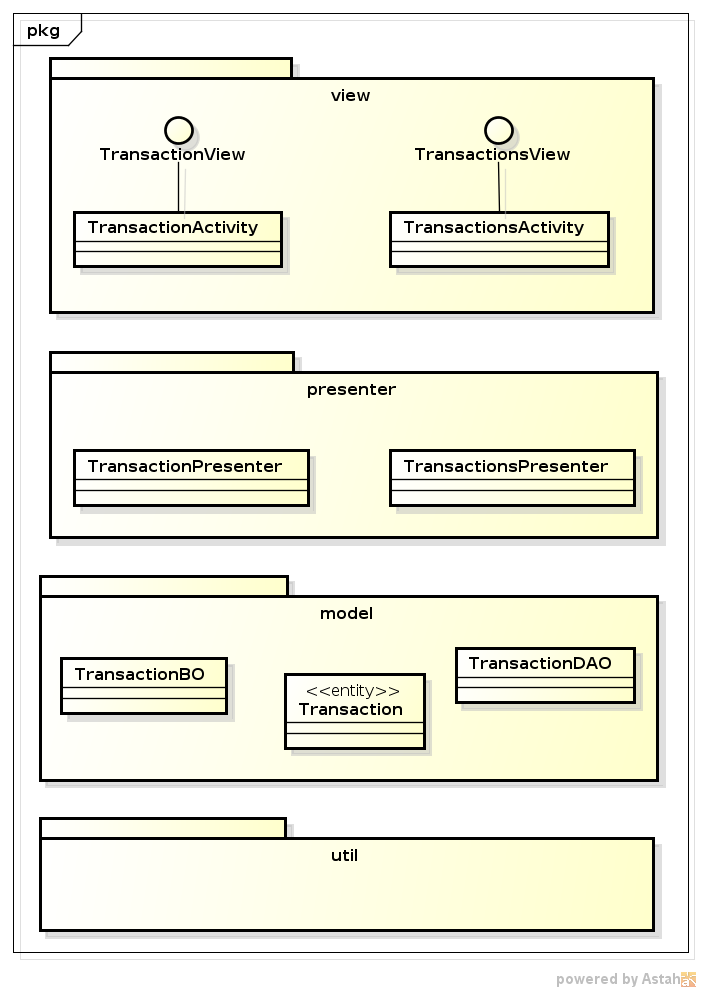
\includegraphics[scale=0.5]{img/arq_poc1.png}
	\caption{Arquitetura POC1/Fonte: Próprio Autor}
	\label{arq_poc1}
\end{figure}

%Como DP resolvem problemas, seguir linha de raciocinio para aplicar padrões em
%android.


\if
Referenciar DIT criticando as heranças das classes da api android

Analise do componente Activity, UI Thread, hieráriquia de herança e algumas
funcionalidades que dependem da activity e como isso interfere na aplicação do
padrão(Por experiência confirmo que é negativa). mostrar exemplo de uma view em
lista para smartphone e outra para tablet com grid usando o mesmo modelo


Experimentos


activity - controller+async task - observer pattern,
activity - controller+async task - localbroadcast

Padrões Criacionais. O objeto Application é um singleton, a activity e
fragmentos são criados pelo android e fica dificil aplicar padrões criacionais é
possível identificar o padrão templete method nos ciclos de vida desses
componentes.



OnTouchListener pode exercer papel de controller pois
pode ser usado para interpretar os gestos do usuário e direcioar para o model.


Quem vai ser o model?

\begin{center}
\begin{tabular}{ | l | l | l | }
  \hline                        
  	Model & View & Presenter \\  \hline
  	Dao & Activity & POJO \\  \hline
\end{tabular}
\end{center}





evitar que outras classes da camada abaixo dependam das classe de view do
android.

%Explicar uso do padrão observer no mvc
Na definição clássica do padrão MVC é possível identificar a implementação do
padrão Observer usado para a comunicação entre o model e a view.


%segunda arquitetura

Observer=Lapsed listener problem=memory leak e bugs porque uma activity pode ser
ou estar sendo referenciada por um listener que se não for desregistrado vai
causar problema

Destacar problema com o observer pattern e pra solucionar isso
usar publish–subscribe messaging pattern

O Broadcast Receiver é uma implementação do padrão pubsub onde diversos
subscribers se registram para receber mensagens(intents) de seu interesse.
\fi





 Para concluir a seção sobre MVC e MVP destacar que A principal características
 desses padrões de projetos é que ele promover maior coesão nos citar Tom deMarco 

baseado em outras pesquisa será aplicado padões de projetos  para melhorar a
 qualidade pegar referências,  relacionar Coesão = Qualidade.


